\documentclass{standalone}
\usepackage{graphics}
\usepackage{tikz}
\pgfrealjobname{survey}
\usepackage{pgfplots}
\usepackage{amsmath}

\begin{document}

\beginpgfgraphicnamed{RZASNodesRadius}
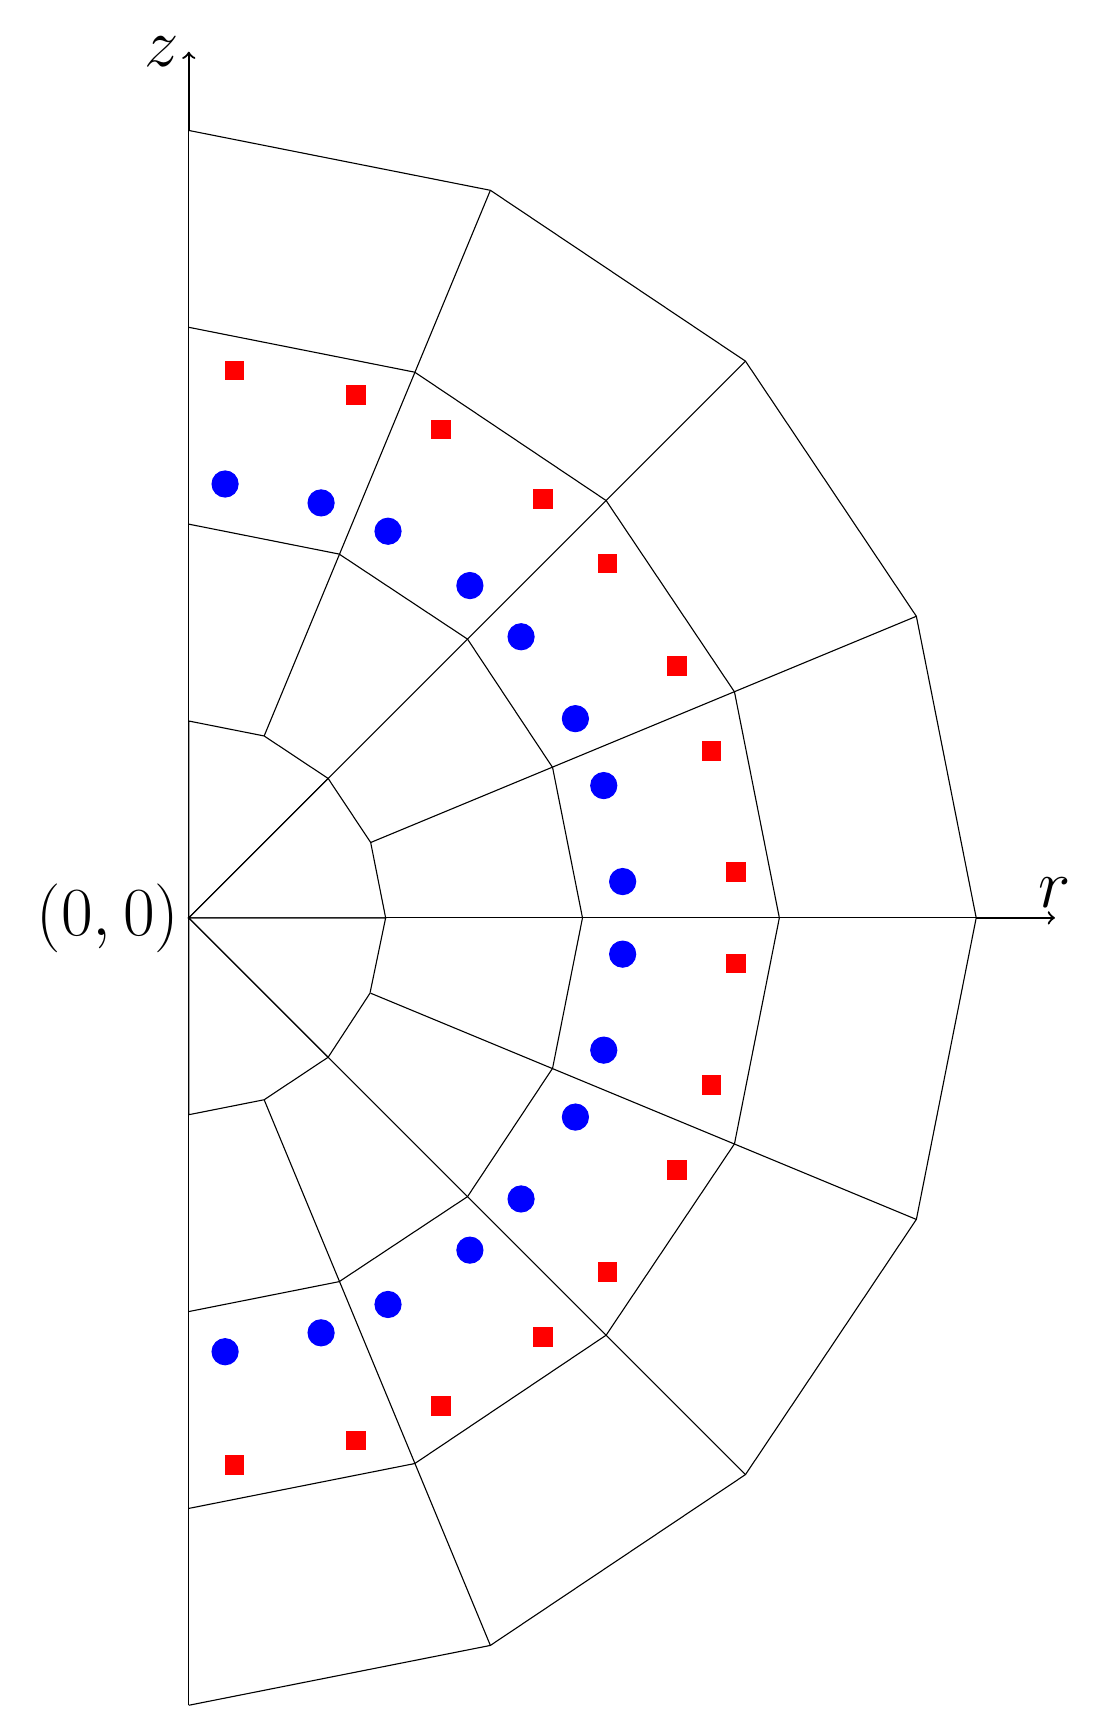
\begin{tikzpicture}
% innermost
\draw (0,0) node[anchor=east]{\Huge $(0,0)$} -- (0,2.5) -- (0.957,2.31) -- (1.77,1.77) -- cycle;
\draw (0,0) -- (1.77,1.77) -- (2.31,0.957) -- (2.5,0) -- cycle;
\draw (0,0) -- (2.5,0) -- (2.301,-0.957) -- (1.77,-1.77) -- cycle;
\draw (0,0) -- (1.77,-1.77) -- (0.957,-2.31) -- (0,-2.5) -- cycle;
% fingers radially outward
\draw (0,2.5) -- (0,10);
\draw[thick,->] (0,10) -- (0,11) node[anchor=east]{\Huge $z$};
\draw (0.957,2.31) -- (3.83,9.24);
\draw (1.77,1.77) -- (7.07,7.07);
\draw (2.31,0.957) -- (9.24,3.83);
\draw (2.5,0) -- (10,0);
\draw[thick,->] (10,0) -- (11,0) node[anchor=south]{\Huge $r$};
\draw (2.31,-0.957) -- (9.24,-3.83);
\draw (1.77,-1.77) -- (7.07,-7.07);
\draw (0.957,-2.31) -- (3.83,-9.24);
\draw (0,-2.5) -- (0,-10);
% 2nd row
\draw (0,5) -- (1.91,4.62) -- (3.54,3.54) -- (4.62,1.91) -- (5,0) -- (4.62,-1.91) -- (3.54,-3.54) -- (1.91,-4.62) -- (0,-5);
% 3rd row
\draw (0,7.5) -- (2.87,6.93) -- (5.30,5.30) -- (6.93,2.87) -- (7.5,0) -- (6.93,-2.87) -- (5.30,-5.30) -- (2.87,-6.93) -- (0,-7.5);
% 4th row
\draw (0,10) -- (3.83,9.24) -- (7.07,7.07) -- (9.24,3.83) -- (10,0) -- (9.24,-3.83) -- (7.07,-7.07) -- (3.83,-9.24) -- (0,-10);

% NODES
% inner row
\node[] at (0.332,0.802){};
0.12643016	0.15994925	0.20388317
0.023701578	0.20250082	0.20388317
0.089859987	0.2169412	0.23481546
0.080239931	0.033236467	0.086851075
0.20250082	0.023701578	0.20388317
0.15994925	0.12643016	0.20388317
0.2169412	0.089859987	0.23481546
0.080239931	-0.033236467	0.086851075
0.15994925	-0.12643016	0.20388317
0.20250082	-0.023701578	0.20388317
0.2169412	-0.089859987	0.23481546
0.033236467	-0.080239931	0.086851075
0.023701578	-0.20250082	0.20388317
0.12643016	-0.15994925	0.20388317
0.089859987	-0.2169412	0.23481546

%  2nd row
0.025246916	0.3017645	0.30281879
0.092155166	0.28845562	0.30281879
0.037280281	0.44559364	0.44715044
0.13607882	0.42594139	0.44715044
0.13880538	0.26913247	0.30281879
0.19552746	0.23123199	0.30281879
0.20496379	0.3974083	0.44715044
0.28872115	0.34144343	0.44715044
0.23123199	0.19552746	0.30281879
0.26913247	0.13880538	0.30281879
0.34144343	0.28872115	0.44715044
0.3974083	0.20496379	0.44715044
0.28845562	0.092155166	0.30281879
0.3017645	0.025246916	0.30281879
0.42594139	0.13607882	0.44715044
0.44559364	0.037280281	0.44715044
0.3017645	-0.025246916	0.30281879
0.28845562	-0.092155166	0.30281879
0.44559364	-0.037280281	0.44715044
0.42594139	-0.13607882	0.44715044
0.26913247	-0.13880538	0.30281879
0.23123199	-0.19552746	0.30281879
0.3974083	-0.20496379	0.44715044
0.34144343	-0.28872115	0.44715044
0.19552746	-0.23123199	0.30281879
0.13880538	-0.26913247	0.30281879
0.28872115	-0.34144343	0.44715044
0.20496379	-0.3974083	0.44715044
0.092155166	-0.28845562	0.30281879
0.025246916	-0.3017645	0.30281879
0.13607882	-0.42594139	0.44715044
0.037280281	-0.44559364	0.44715044

% 3rd row
\node[draw,circle,blue,fill=blue] at (0.46089315,5.51){};
\node[draw,circle,blue,fill=blue] at (1.68,5.27){};
\node[draw,mark=square,red,fill=red] at (0.581,6.95){};
\node[draw,mark=square,red,fill=red] at (2.12,6.64){};
\node[draw,circle,blue,fill=blue] at (2.53,4.91){};
\node[draw,circle,blue,fill=blue] at (3.57,4.22){};
\node[draw,mark=square,red,fill=red] at (3.20,6.20){};
\node[draw,mark=square,red,fill=red] at (4.50,5.32){};
\node[draw,circle,blue,fill=blue] at (4.22,3.57){};
\node[draw,circle,blue,fill=blue] at (4.91,2.53){};
\node[draw,mark=square,red,fill=red] at (5.32,4.50){};
\node[draw,mark=square,red,fill=red] at (6.20,3.20){};
\node[draw,circle,blue,fill=blue] at (5.27,1.68){};
\node[draw,circle,blue,fill=blue] at (5.51,0.461){};
\node[draw,mark=square,red,fill=red] at (6.64,2.12){};
\node[draw,mark=square,red,fill=red] at (6.95,0.581){};
\node[draw,circle,blue,fill=blue] at (5.51,-0.461){};
\node[draw,circle,blue,fill=blue] at (5.27,-1.68){};
\node[draw,mark=square,red,fill=red] at (6.95,-0.581){};
\node[draw,mark=square,red,fill=red] at (6.64,-2.12){};
\node[draw,circle,blue,fill=blue] at (4.91,-2.53){};
\node[draw,circle,blue,fill=blue] at (4.22,-3.57){};
\node[draw,mark=square,red,fill=red] at (6.20,-3.20){};
\node[draw,mark=square,red,fill=red] at (5.32,-4.50){};
\node[draw,circle,blue,fill=blue] at (3.57,-4.22){};
\node[draw,circle,blue,fill=blue] at (2.53,-4.91){};
\node[draw,mark=square,red,fill=red] at (4.50,-5.32){};
\node[draw,mark=square,red,fill=red] at (3.20,-6.20){};
\node[draw,circle,blue,fill=blue] at (1.68,-5.27){};
\node[draw,circle,blue,fill=blue] at (0.461,-5.51){};
\node[draw,mark=square,red,fill=red] at (2.12,-6.64){};
\node[draw,mark=square,red,fill=red] at (0.581,-6.95){};

% 4th row
0.066931714	0.80000327	0.80279828
0.24431116	0.7647203	0.80279828
0.078965078	0.94383241	0.94712993
0.28823481	0.90220607	0.94712993
0.36798484	0.71349299	0.80279828
0.51835987	0.6130156	0.80279828
0.43414325	0.84176882	0.94712993
0.61155355	0.72322704	0.94712993
0.6130156	0.51835987	0.80279828
0.71349299	0.36798484	0.80279828
0.72322704	0.61155355	0.94712993
0.84176882	0.43414325	0.94712993
0.7647203	0.24431116	0.80279828
0.80000327	0.066931714	0.80279828
0.90220607	0.28823481	0.94712993
0.94383241	0.078965078	0.94712993
0.80000327	-0.066931714	0.80279828
0.7647203	-0.24431116	0.80279828
0.94383241	-0.078965078	0.94712993
0.90220607	-0.28823481	0.94712993
0.71349299	-0.36798484	0.80279828
0.6130156	-0.51835987	0.80279828
0.84176882	-0.43414325	0.94712993
0.72322704	-0.61155355	0.94712993
0.51835987	-0.6130156	0.80279828
0.36798484	-0.71349299	0.80279828
0.61155355	-0.72322704	0.94712993
0.43414325	-0.84176882	0.94712993
0.24431116	-0.7647203	0.80279828
0.066931714	-0.80000327	0.80279828
0.28823481	-0.90220607	0.94712993
0.078965078	-0.94383241	0.94712993


\end{tikzpicture}
\endpgfgraphicnamed

\end{document}